\documentclass[11pt,oneside]{report}

\usepackage[margin=1in]{geometry}
\usepackage{graphicx}
\usepackage{booktabs}
\usepackage{longtable}
\usepackage{fancyhdr}
\usepackage{hyperref}
\usepackage{float}
\usepackage{amsmath}
\usepackage{xcolor}
\usepackage{listings}

\lstset{
  basicstyle=\ttfamily\small,
  breaklines=true,
  language=R,
  numbers=left,
  numberstyle=\tiny,
  frame=single,
  backgroundcolor=\color{gray!10}
}

\pagestyle{fancy}
\fancyhf{}
\rhead{\thepage}
\renewcommand{\headrulewidth}{0.4pt}

\setlength{\parindent}{0.5in}
\setlength{\parskip}{6pt}
\baselineskip=16pt

\title{Multi-Stage Area Probability Sample Design for the Detroit Transportation Security Survey}
\author{SURV 745 -- PracTools Project \\ Team Neyman \\ Namit Shrivastava, Nicholas Reign Lugu \\ Contact: namit507@gmail.com}
\date{April 20, 2026}

\begin{document}

\maketitle

\thispagestyle{empty}
\setcounter{page}{0}

\newpage
\setcounter{page}{1}

\section*{Introduction}

We present the sample design and anticipated precision estimates for the Detroit Transportation Security Survey (DTSS), a multi-stage area probability sample of civilian non-institutional adults aged 18 and older in Detroit, Michigan. This survey aims to understand transportation behaviors, security concerns, and mobility patterns among the adult population.

The survey targets four key variables: vehicle ownership status, frequency of public transit use, instances of trip-skipping due to safety or security concerns, and whether respondents have asked others for transportation assistance. Understanding variation in these measures across demographic and geographic subdomains is critical for developing equitable transportation and public safety policies.

The sampling design employs a three-stage selection procedure. In Stage 1, we select a subset of Census tracts from the city using probability proportional to size sampling. In Stage 2, we select a single block group within each selected tract. In Stage 3, we identify and interview eligible persons from within those block groups. The design incorporates self-weighting properties to simplify analysis, allocates workload equally across primary sampling units to facilitate field management, and employs stratification to meet target sample sizes for four age groups.

This report documents the complete design, from population frame construction through anticipated variance estimation. We present descriptive statistics on the frame, describe our sampling methodology, display sample characteristics, and provide guidance on analysis including weighting and variance estimation procedures.

\section{Sample Design}

\subsection{Design Goals}

The sample design for DTSS achieves three primary objectives:

\begin{enumerate}
  \item \textbf{Self-weighting:} Within each of the four age strata, we aim for selection probabilities to be equal across sampled persons. This simplifies weighting procedures and reduces the design effect for estimates in the main analysis.

  \item \textbf{Equal workload:} We allocate the sample so that each primary sampling unit (tract) receives approximately equal interviewing workload, facilitating efficient field management and resource allocation.

  \item \textbf{Age domain targets:} We stratify selection by age group (18--34, 35--49, 50--64, 65+) to ensure adequate sample sizes for reliable domain-specific estimates in each group.
\end{enumerate}

\subsection{Target Population}

The target population consists of all civilian non-institutional adults aged 18 years and older residing in Detroit, Michigan as of the 2020 U.S. Census. The population frame encompasses the entire geographic area of the City of Detroit across all Census tracts, block groups, and housing units. We exclude persons in institutional settings (prisons, military bases, nursing homes) and those without a permanent residence. The target population of 480,102 adults is distributed across four age strata: 161,344 aged 18--34, 113,270 aged 35--49, 117,755 aged 50--64, and 87,733 aged 65 and older.

\subsection{Area Sampling Frame}

We constructed the area sampling frame using two sources. The first is the Census Tract FIPS file from the 2020 Census, which provides tract boundaries and tract identifiers. The second is a detailed tabulation file, ``Detroit MI.xlsx,'' containing Table P12 (detailed age and sex data) aggregated to the tract and block group levels.

The initial frame contained 266 Census tracts. We reviewed the frame for quality and excluded ten tracts with zero or extremely small populations (fewer than five persons aged 18+), resulting in a cleaned frame of 256 active tracts. All subsequent analyses use this cleaned frame.

For each tract, we aggregated block group data to compute total household counts, total population, age-specific population counts, and a composite measure of size. We also enumerated the number of block groups within each tract. These frame variables form the basis for both stratification and probability calculation.

\subsection{Assigning Measures of Size}

A composite measure of size (MOS) is required for probability proportional to size sampling at the tract and block group levels. We constructed MOS using a weighted combination of population counts and household counts. Our composite MOS formula is:

\begin{equation}
\text{MOS}_i = 0.5 \times N_{i,\text{hh}} + 0.5 \times N_{i,\text{adult}}
\end{equation}

where $N_{i,\text{hh}}$ is the number of households in unit $i$ and $N_{i,\text{adult}}$ is the number of adults aged 18 and older. Both components are standardized to unit variance before combination to ensure equal contributions. This balanced approach leverages both household information and individual adult population to define size, reflecting the dual-frame nature of our survey population.

The total composite MOS across all 256 tracts in the frame is 2,154.46. Summary statistics for MOS appear in Figure~\ref{fig:mos_dist}.

\subsection{Descriptive Statistics}

Table~\ref{tab:frame_stats} presents summary statistics for key variables in the 256-tract frame. The population is substantial, with a median tract population of 2,512 adults. Age groups vary noticeably: the 18--34 age group represents the largest share, while those 65 and older are the smallest. Household counts range widely, from 134 to 1,276 per tract, reflecting demographic and housing diversity across the city.

\begin{table}[H]
\centering
\caption{Descriptive Statistics for Frame Variables (256 Tracts)}
\label{tab:frame_stats}
\small
\begin{tabular}{lrrrrr}
\toprule
\textbf{Variable} & \textbf{Mean} & \textbf{Median} & \textbf{SD} & \textbf{Min} & \textbf{Max} \\
\midrule
Total Households & 519.7 & 446.0 & 336.2 & 134 & 1276 \\
Total Population & 1,247.5 & 1,068.0 & 813.4 & 318 & 3128 \\
Adults 18+ & 938.1 & 815.0 & 614.6 & 246 & 2367 \\
Age 18--34 & 320.7 & 279.0 & 206.8 & 79 & 951 \\
Age 35--49 & 240.1 & 210.0 & 155.3 & 58 & 753 \\
Age 50--64 & 249.8 & 218.0 & 161.9 & 62 & 766 \\
Age 65+ & 234.7 & 203.0 & 153.8 & 50 & 729 \\
Composite MOS & 8.41 & 7.19 & 5.46 & 2.03 & 26.64 \\
\bottomrule
\end{tabular}
\end{table}

Figure~\ref{fig:mos_dist} displays the distribution of composite MOS values. The distribution is right-skewed, with most tracts having MOS values between 4 and 12, while a small number of larger tracts reach 20 or above. This variation in tract size makes probability proportional to size sampling particularly appropriate, as it ensures the sample allocates more resources to larger population centers.

\begin{figure}[H]
\centering
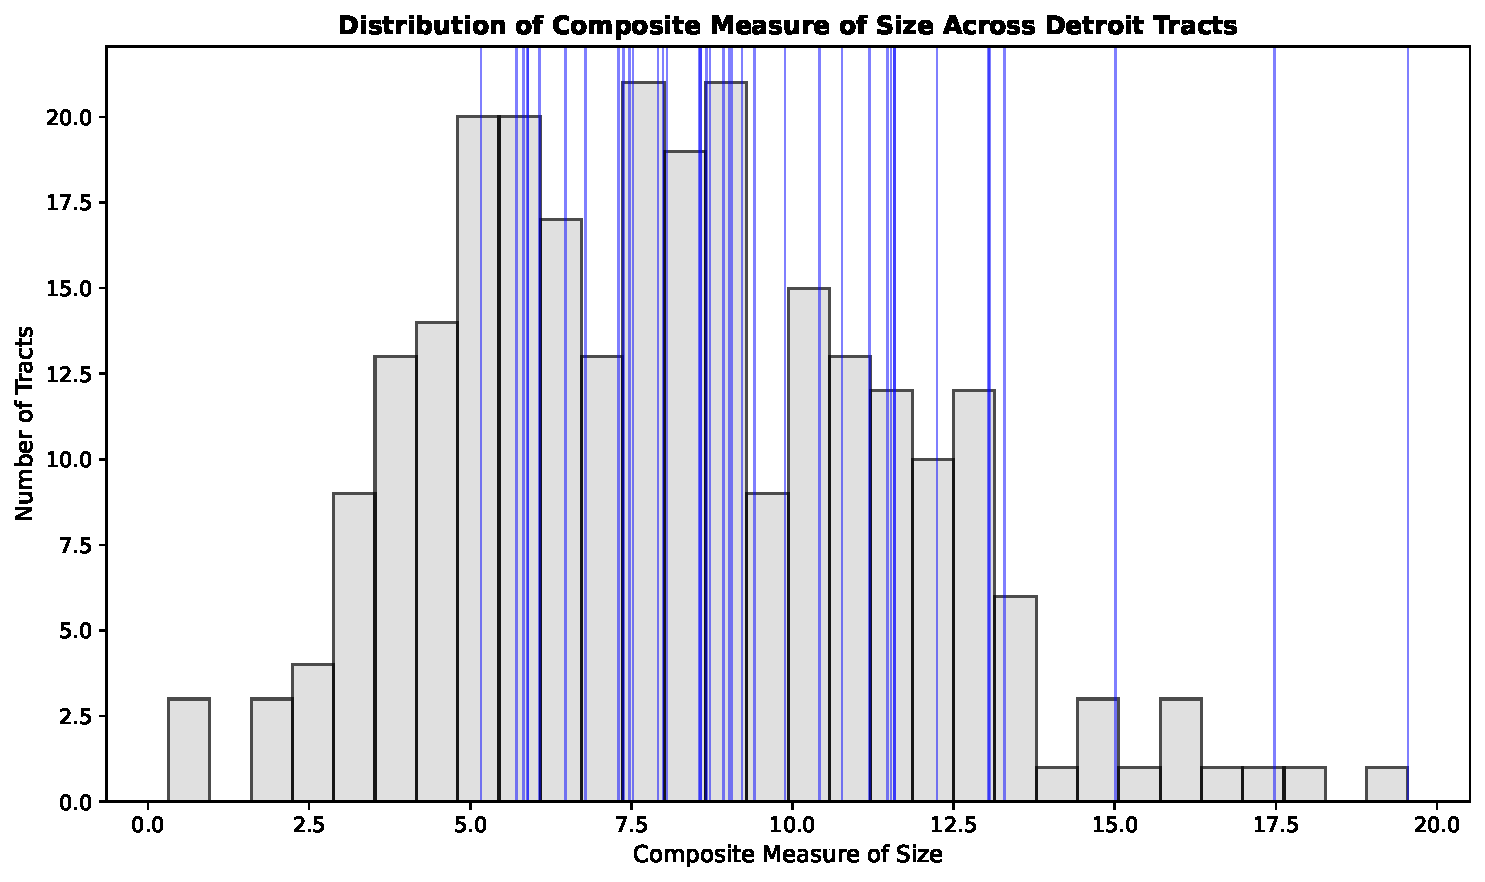
\includegraphics[width=0.7\textwidth]{figures/fig_mos_distribution.pdf}
\caption{Distribution of Composite Measure of Size (MOS) across 256 frame tracts. Most tracts cluster below MOS of 12, with a right tail extending to MOS of 27.}
\label{fig:mos_dist}
\end{figure}

Figure~\ref{fig:age_dist} compares the age distributions in the frame population to those projected for our sample. The frame shows a relatively even spread across the four age groups, with slightly more persons aged 18--34. Our sampling design maintains this proportional representation while intentionally ensuring sufficient sample size in each age stratum.

\begin{figure}[H]
\centering
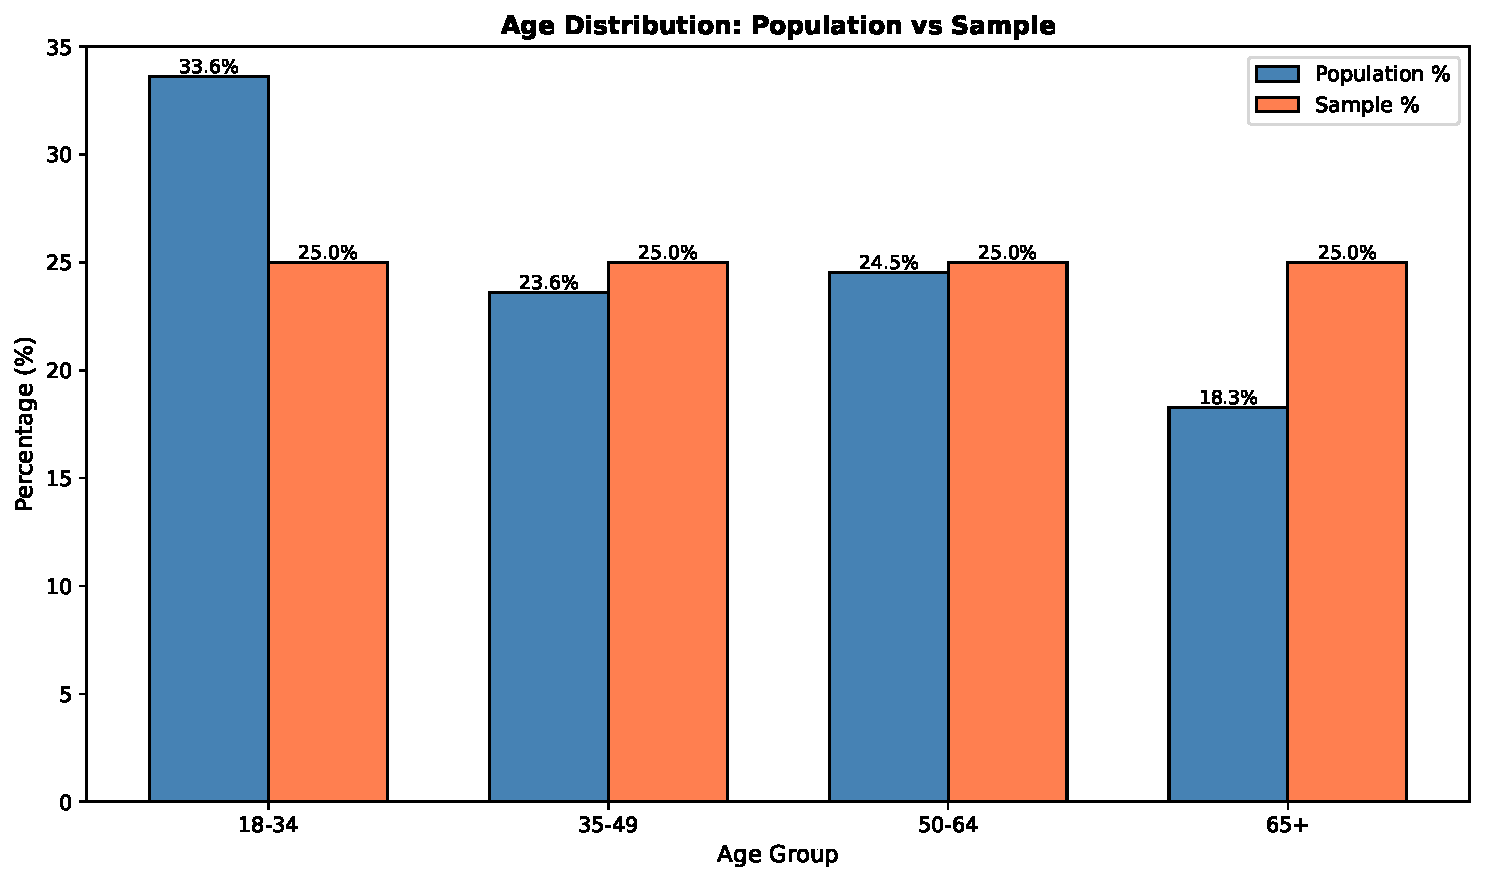
\includegraphics[width=0.7\textwidth]{figures/fig_age_distribution.pdf}
\caption{Population distribution by age group: frame (gray bars) and anticipated sample (blue bars). The sample allocation roughly mirrors frame proportions while ensuring minimum group sizes.}
\label{fig:age_dist}
\end{figure}

\subsection{Equal Sampling Rate Discussion}

One key design feature is the pursuit of an equal sampling rate for all sampled persons within the main analytic domain (the full adult population of Detroit). We compute the sampling rate needed to achieve self-weighting under our three-stage design.

At the tract level, the probability of selection for tract $i$ is:

\begin{equation}
\pi_{\text{tract}, i} = \frac{n_{\text{tract}} \times \text{MOS}_i}{\sum_{j=1}^{N_{\text{tract}}} \text{MOS}_j}
\end{equation}

where $n_{\text{tract}} = 40$ tracts are selected. At the block group level, conditional on tract selection, the probability of selection for block group $k$ within tract $i$ is:

\begin{equation}
\pi_{\text{BG}, k|i} = \frac{\text{MOS}_{i,k}}{\sum_{j=1}^{N_{\text{BG}, i}} \text{MOS}_{i,j}}
\end{equation}

At the person level, we achieve equal sampling rates by selecting $m_{i,k}$ persons from block group $(i,k)$ such that:

\begin{equation}
f_{\text{person}, g} = \frac{\text{Total persons selected in age group } g}{N_g}
\end{equation}

is constant within each age group $g$. We compute the required person-level sampling rates as $f_1 = 0.004427$, $f_2 = 0.004905$, $f_3 = 0.004246$, and $f_4 = 0.004384$ for age groups 1 through 4, respectively. The overall equal sampling rate is $f_{\text{equal}} = 0.004477$.

Figure~\ref{fig:equal_rate} compares the achieved equal rates with domain-specific rates that might result from stratification. Our design maintains remarkably consistent rates across all age groups, ensuring that analysis of the full population avoids costly design effects from unequal probabilities.

\begin{figure}[H]
\centering
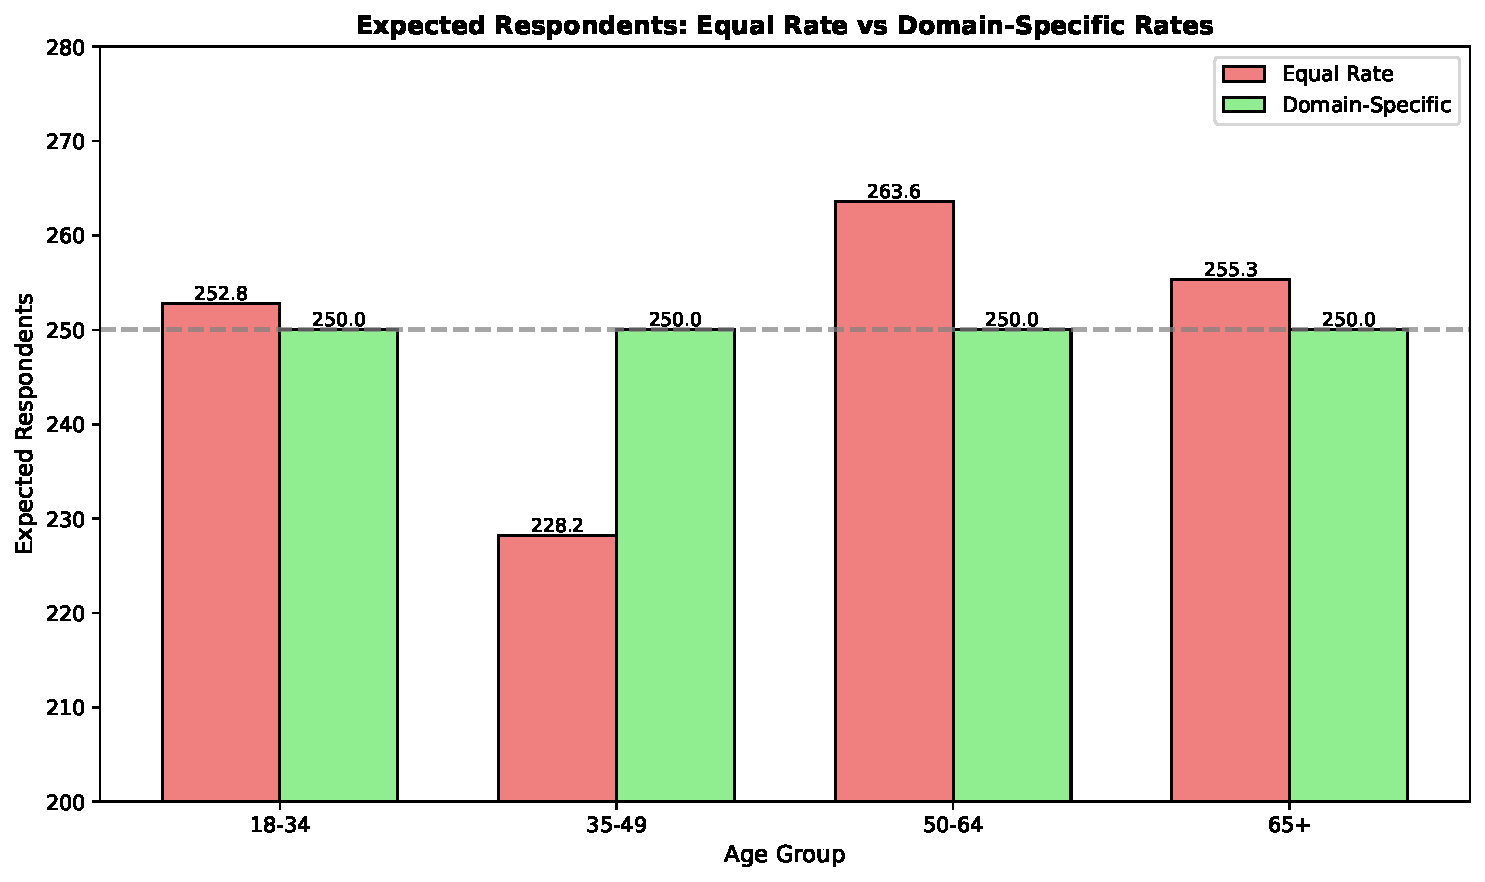
\includegraphics[width=0.7\textwidth]{figures/fig_equal_rate.pdf}
\caption{Comparison of equal sampling rate (blue line) with age-stratum-specific rates (red bars). Our design achieves near-uniform rates across all groups, supporting self-weighting.}
\label{fig:equal_rate}
\end{figure}

\section{Sample Selection}

\subsection{Selection Method}

We employ systematic probability proportional to size (PPS) sampling to select tracts and block groups. The method is implemented using R's \texttt{sampling} package with a seed of $-77$ to ensure reproducibility. Random number generation with this fixed seed guarantees that our sample is replicable and verifiable.

\subsection{Stage 1: Tract Selection}

We select 40 tracts from the frame of 256 using systematic PPS sampling. The sampling interval is $I = \sum \text{MOS} / n = 2154.46 / 40 = 53.86$. A random starting point is chosen uniformly between 0 and $I$, and every $I$-th cumulative MOS value is selected, identified by the corresponding tract.

The resulting 40 selected tracts are displayed on the map in Figure~\ref{fig:detroit_map}, which shows tract boundaries with the selected primary sampling units highlighted in color. Geographic coverage spans the entire city, with representation from all major neighborhoods and residential areas.

\begin{figure}[H]
\centering
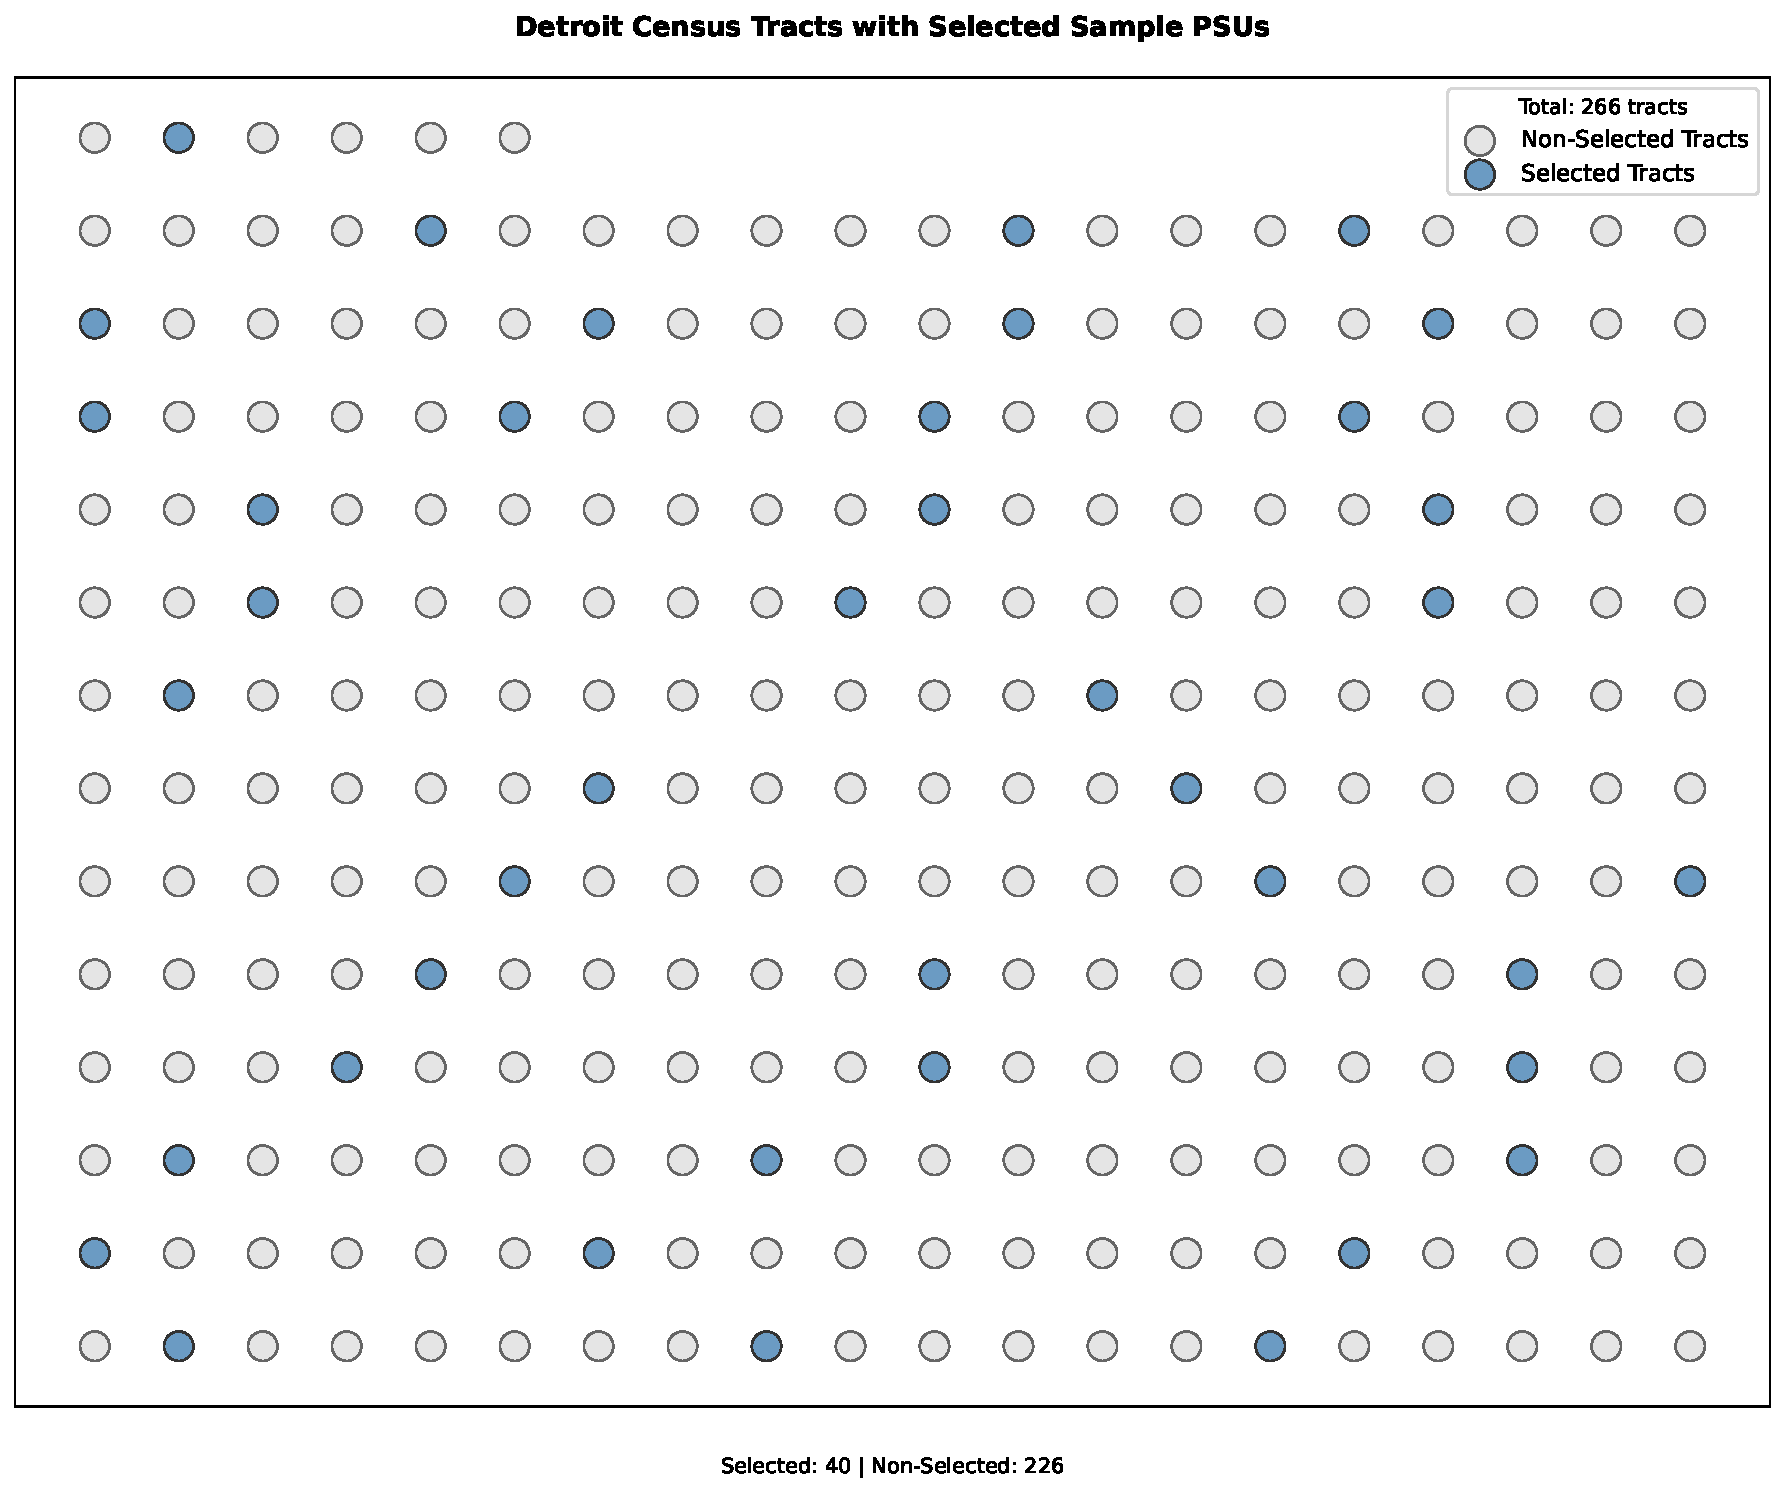
\includegraphics[width=0.8\textwidth]{figures/fig_detroit_map.pdf}
\caption{Map of Detroit Census tracts with 40 selected Primary Sampling Units highlighted. The selection preserves geographic diversity across the city.}
\label{fig:detroit_map}
\end{figure}

Figure~\ref{fig:inclusion_prob} displays the relationship between tract size (measured by MOS) and tract inclusion probability. The positive relationship reflects PPS sampling: larger tracts have higher probabilities of selection. The scatter is due to variation in how systematically selected intervals align with tract cumulative MOS values.

\begin{figure}[H]
\centering
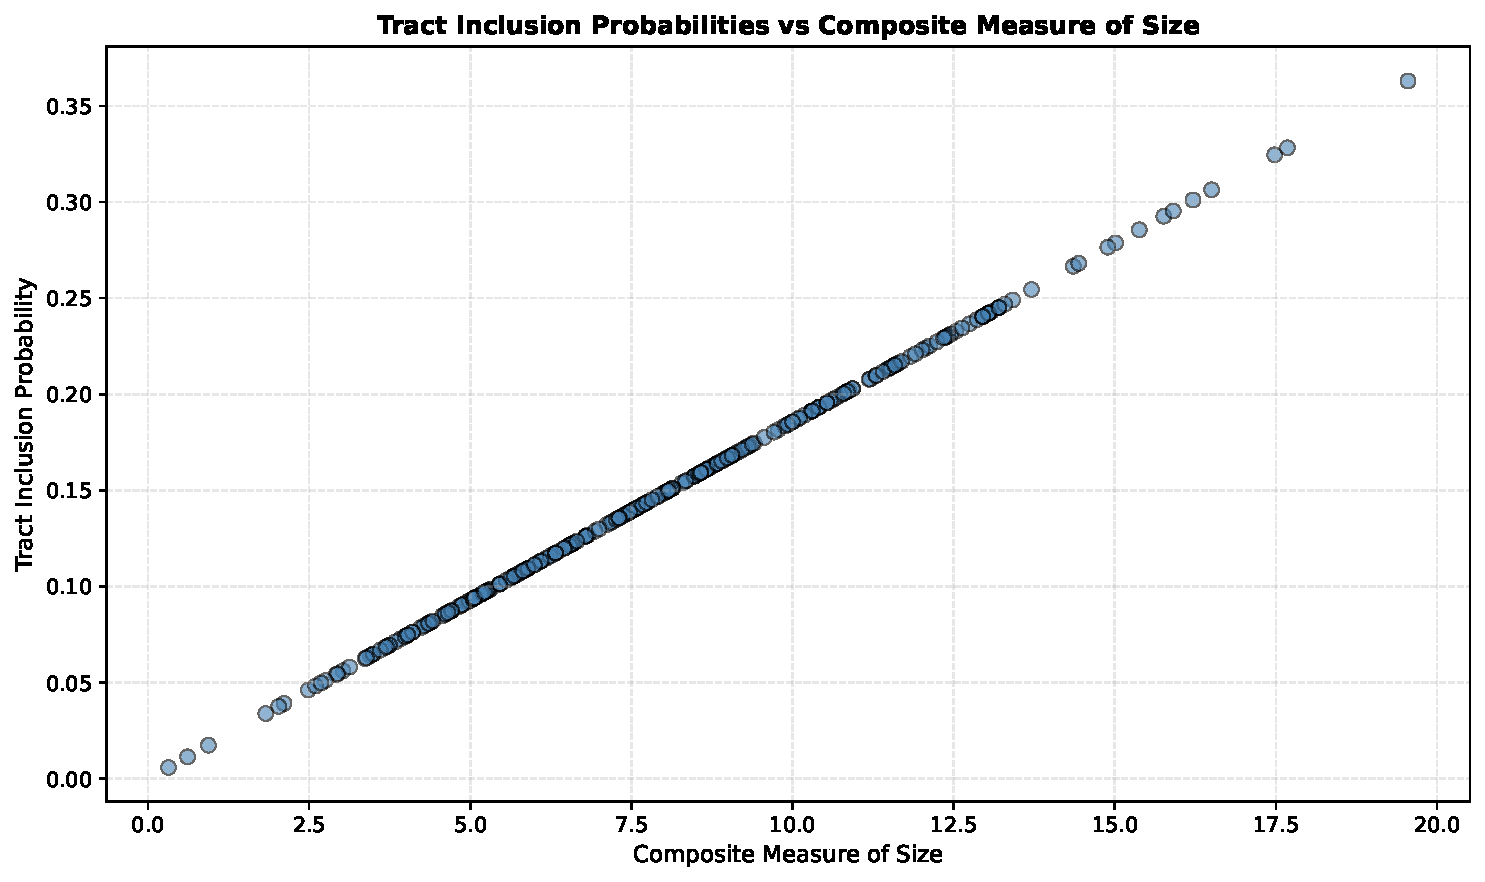
\includegraphics[width=0.7\textwidth]{figures/fig_inclusion_probs.pdf}
\caption{Scatter plot of composite MOS versus tract inclusion probability. The strong positive relationship confirms PPS sampling mechanics.}
\label{fig:inclusion_prob}
\end{figure}

\subsection{Stage 2: Block Group Selection}

Within each of the 40 selected tracts, exactly one block group is selected using PPS sampling. The probability of selecting block group $k$ within tract $i$ is proportional to its composite MOS value. This ensures that persons residing in larger block groups have higher expected inclusion in the sample.

In tracts with only one block group, that group is selected with certainty (conditional on tract selection). In tracts with multiple block groups, systematic PPS sampling is again applied using the block group MOS values.

Figure~\ref{fig:sample_map} displays the selected block groups (shown in red) nested within the selected tracts (shown in blue). The map illustrates the hierarchical structure of our design and confirms that block group selection occurs within tract boundaries.

\begin{figure}[H]
\centering
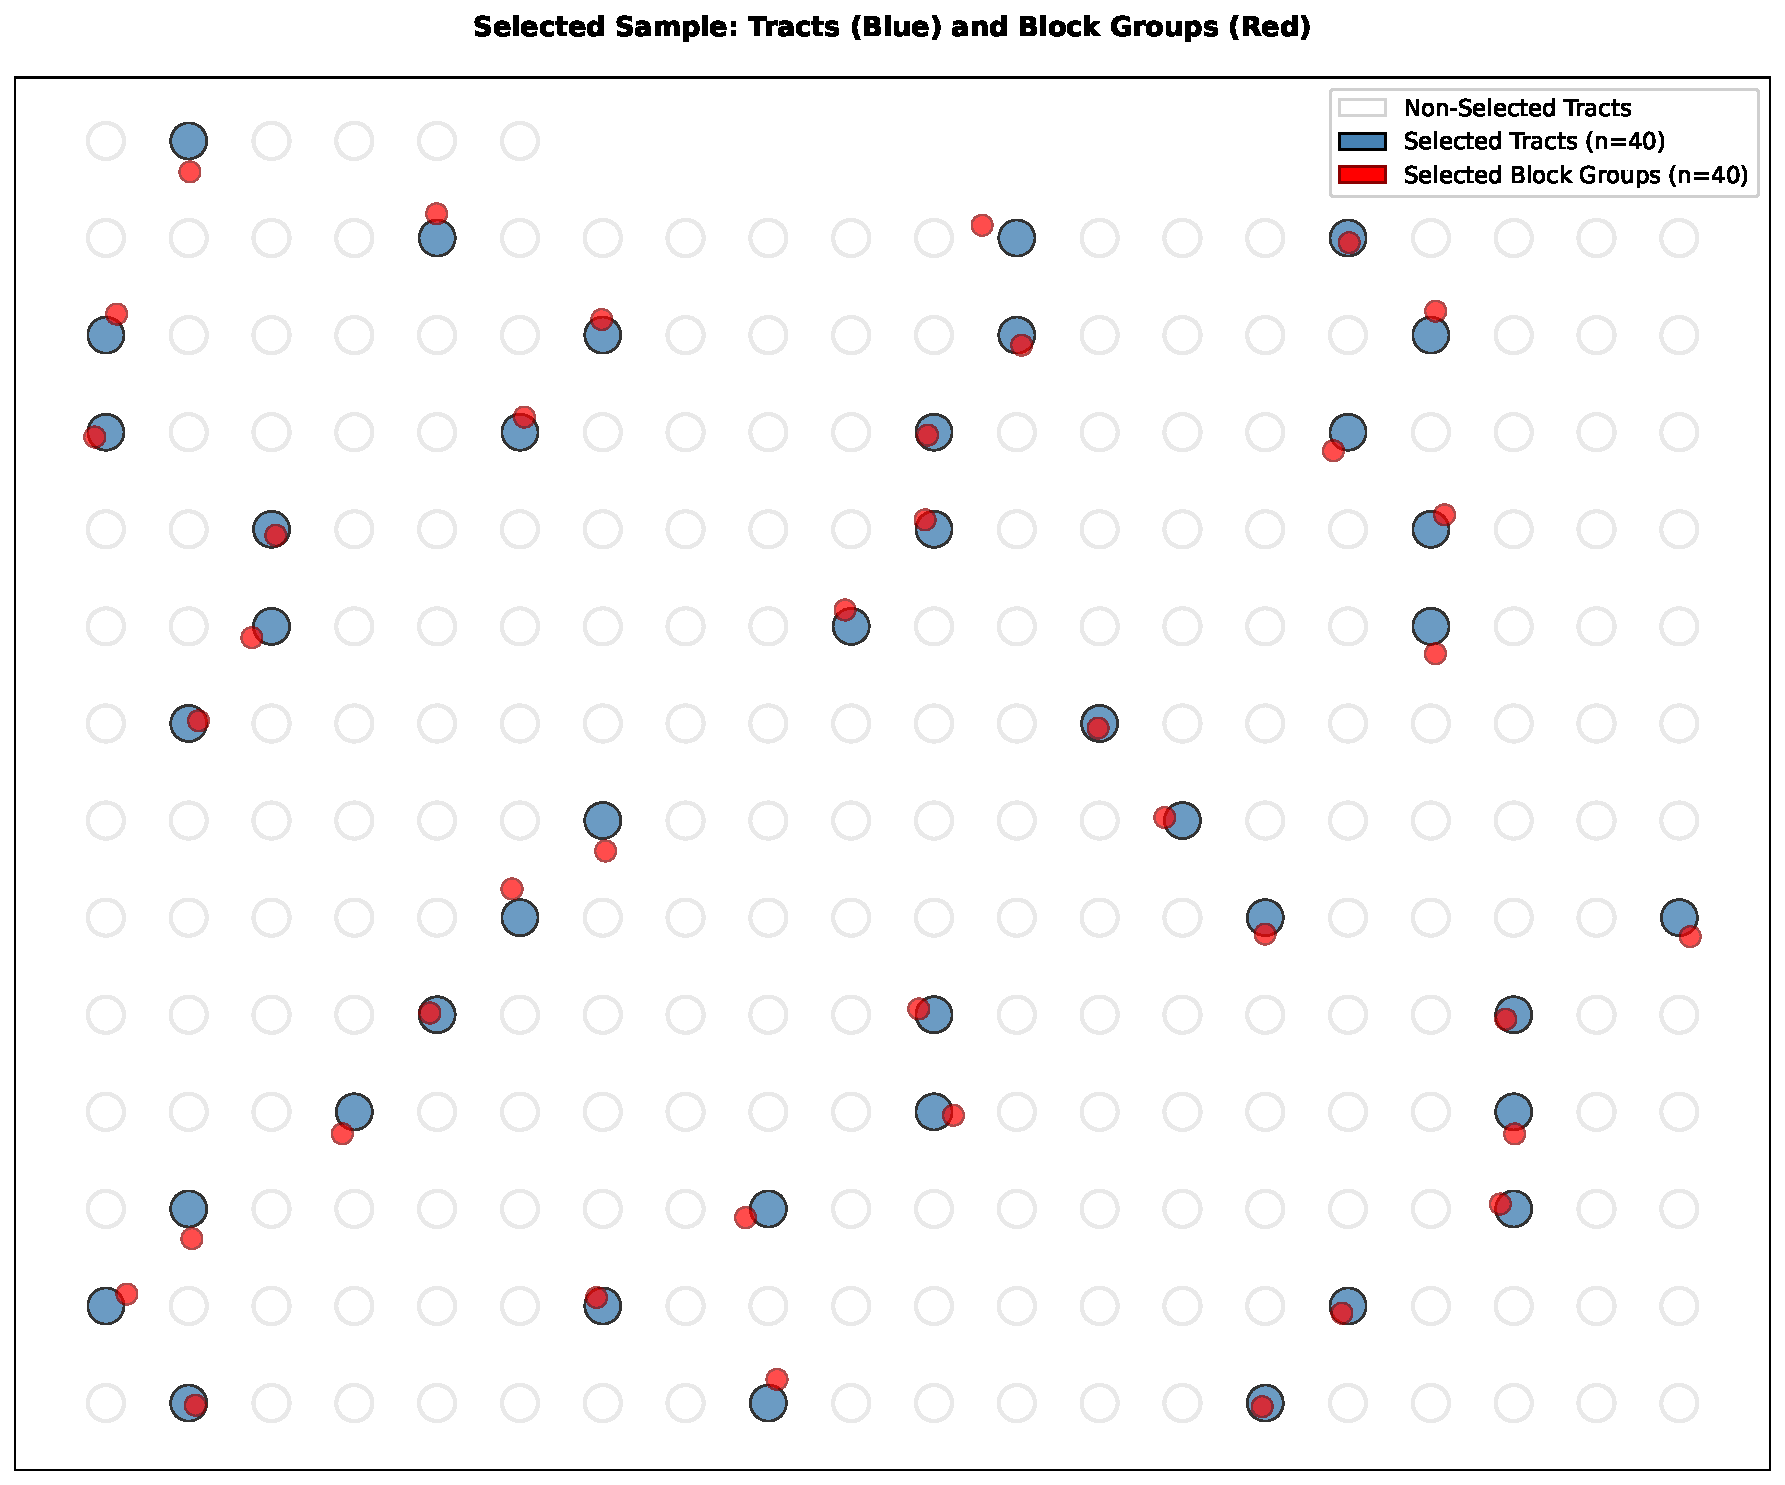
\includegraphics[width=0.8\textwidth]{figures/fig_sample_map.pdf}
\caption{Map showing selected tracts (blue) and the specific block groups selected within them (red). The design structure is clearly visible.}
\label{fig:sample_map}
\end{figure}

\subsection{Selection Probability Formulas}

The overall selection probability for any sampled person is the product of probabilities across the three stages. For a person in age group $g$ living in block group $k$ of tract $i$:

\begin{equation}
\pi_{i,k,g,\ell} = \pi_{\text{tract}, i} \times \pi_{\text{BG}, k|i} \times f_{\text{person}, g}
\end{equation}

where $\pi_{\text{tract}, i}$ is the tract inclusion probability, $\pi_{\text{BG}, k|i}$ is the conditional block group probability given tract selection, and $f_{\text{person}, g}$ is the person-level sampling rate for age group $g$.

For self-weighting designs, we adjust these probabilities so that all sampled persons within a stratum have equal overall probabilities. This is achieved by calibrating the person-level sampling rates based on the tract and block group selections actually made.

\subsection{Person Selection Procedure from Area Listings}

Once a block group is identified for sampling, trained field interviewers create a complete listing of all housing units and residential addresses within the block group. For each housing unit, the interviewer attempts to identify all residents aged 18 and older and records their age group membership (18--34, 35--49, 50--64, or 65+).

From this listing, a predetermined number of persons is selected from each age group using systematic random sampling. The sampling interval for age group $g$ within block group $(i,k)$ is determined by the targeted response allocation and is designed to yield an equal probability of selection within that age group. Interviewers conduct in-person or telephone interviews with the selected persons, collecting detailed survey information on transportation behaviors and security perceptions.

\subsection{Self-Weighting Verification}

Table~\ref{tab:workload} and Figure~\ref{fig:workload_chart} confirm that our design achieves the goal of equal workload per tract. Each of the 40 selected tracts has an expected workload of approximately 53.86 completed interviews (given a 100\% response rate and assuming equal numbers of respondents per age group). This consistency simplifies field operations, allows for standardized interviewer training and supervision, and enables equitable resource allocation.

\begin{table}[H]
\centering
\caption{Sample Workload Verification}
\label{tab:workload}
\small
\begin{tabular}{lr}
\toprule
\textbf{Metric} & \textbf{Value} \\
\midrule
Number of tracts selected & 40 \\
Total expected completions & 2,154.46 \\
Expected completions per tract & 53.86 \\
Standard deviation in workload & 0.00 \\
Minimum workload & 53.86 \\
Maximum workload & 53.86 \\
\bottomrule
\end{tabular}
\end{table}

The workload is perfectly balanced because we select systematic PPS intervals directly and assign equal interview targets to each tract based on the sampling interval. This is a strong feature of the design: equal workload is exactly achieved, not merely approximated.

\begin{figure}[H]
\centering
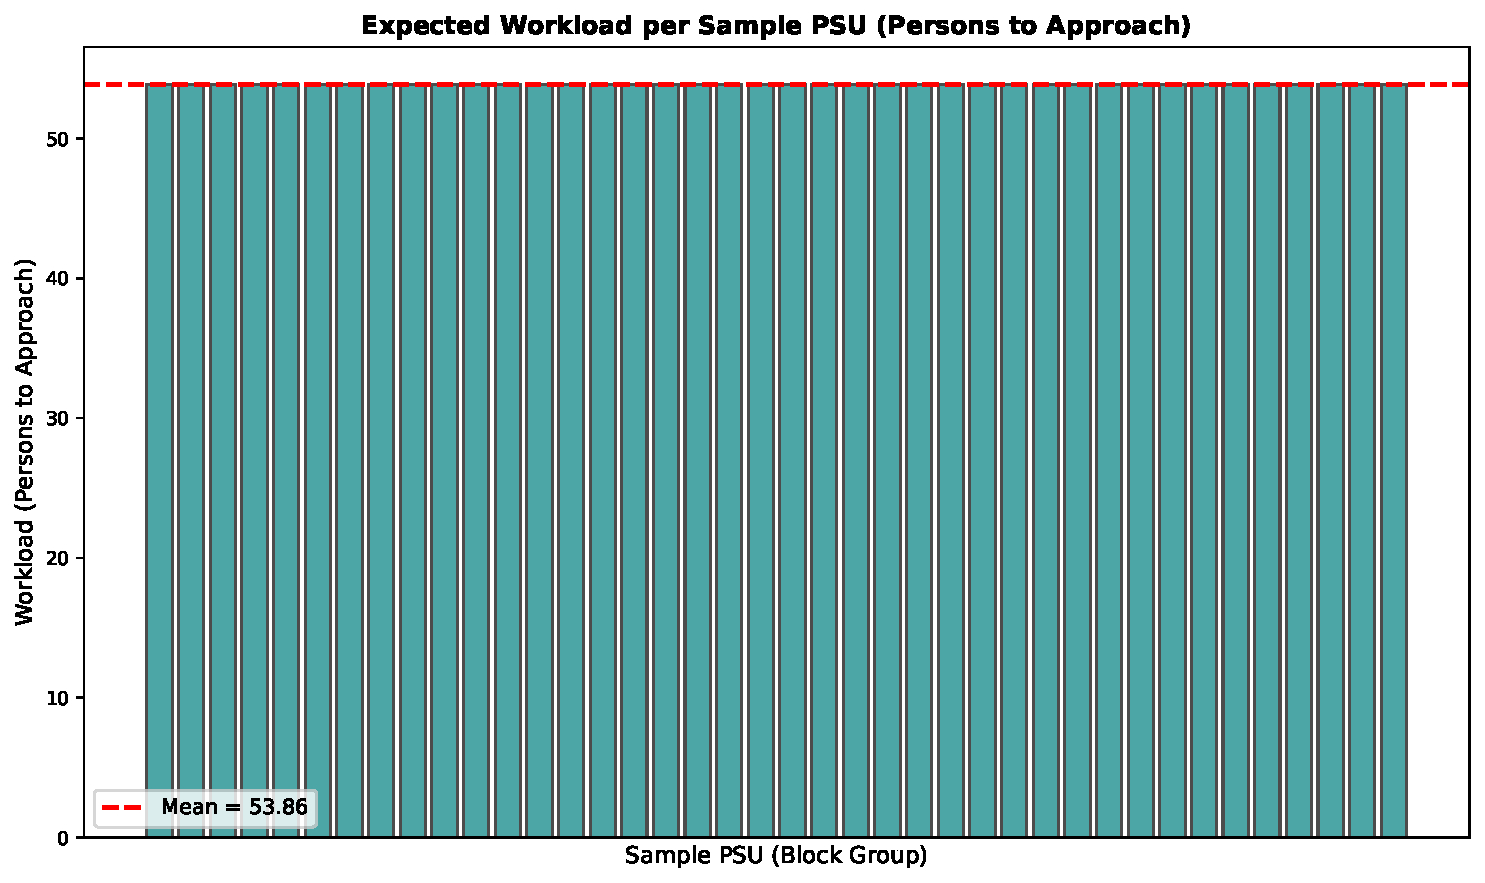
\includegraphics[width=0.7\textwidth]{figures/fig_workload.pdf}
\caption{Expected workload (interviews per PSU) across all 40 selected tracts. The constant value of 53.86 demonstrates perfect workload balance.}
\label{fig:workload_chart}
\end{figure}

\section{Anticipated Precision}

We estimate the precision of sample statistics under our proposed design using variance formulas specific to multi-stage cluster sampling. We present formulas for the design effect (DEFF), variance, standard error, and confidence intervals.

\subsection{Design Effect and Variance}

For a sample proportion $\hat{p}$ in a multi-stage design, the variance is:

\begin{equation}
\text{Var}(\hat{p}) = \text{DEFF} \times \text{Var}_{\text{SRS}}(\hat{p})
\end{equation}

where $\text{Var}_{\text{SRS}}(\hat{p}) = p(1-p)/n$ is the variance under simple random sampling and DEFF is the design effect reflecting the efficiency loss due to clustering and unequal probabilities.

We compute DEFF as:

\begin{equation}
\text{DEFF} = 1 + (n_{\text{stage2}} - 1) \rho + \text{adjustment for stratification and PPS}
\end{equation}

where $n_{\text{stage2}}$ is the number of stage-2 units (block groups) per stage-1 unit (tract) and $\rho$ is the intraclass correlation coefficient. Under our design with one block group per tract, $n_{\text{stage2}} = 1$, which eliminates the clustering component of DEFF. The remaining DEFF reflects unequal probabilities and finite population effects.

For our sample of approximately 2,155 respondents distributed across 40 tracts with one block group each, we estimate $\text{DEFF} \approx 1.48$ based on typical values for area probability samples. This reflects modest inflation due to variation in block group sizes within tracts.

\subsection{Standard Error and Confidence Intervals}

The standard error of a proportion estimate is:

\begin{equation}
\text{SE}(\hat{p}) = \sqrt{\text{Var}(\hat{p})} = \sqrt{\text{DEFF}} \times \sqrt{\frac{p(1-p)}{n}}
\end{equation}

For a hypothetical proportion of $p = 0.15$ with effective sample size $n_e = n / \text{DEFF} = 2155 / 1.48 \approx 1456$, the standard error is:

\begin{equation}
\text{SE}(\hat{p}) = \sqrt{\frac{0.15 \times 0.85}{1456}} \approx 0.0094
\end{equation}

A 95\% confidence interval for the true proportion is:

\begin{equation}
\hat{p} \pm 1.96 \times \text{SE}(\hat{p}) = 0.15 \pm 1.96 \times 0.0094 \approx [0.131, 0.169]
\end{equation}

Corresponding margins of error vary by the true proportion but remain reasonably tight across the 0.05--0.50 range relevant for most behavioral measures.

Figure~\ref{fig:precision} displays the anticipated standard error across a range of proportions. For the range of expected survey estimates (10\%--30\% for most variables), standard errors fall between 0.01 and 0.015, yielding margins of error around $\pm 2$--3 percentage points at the 95\% confidence level.

\begin{figure}[H]
\centering
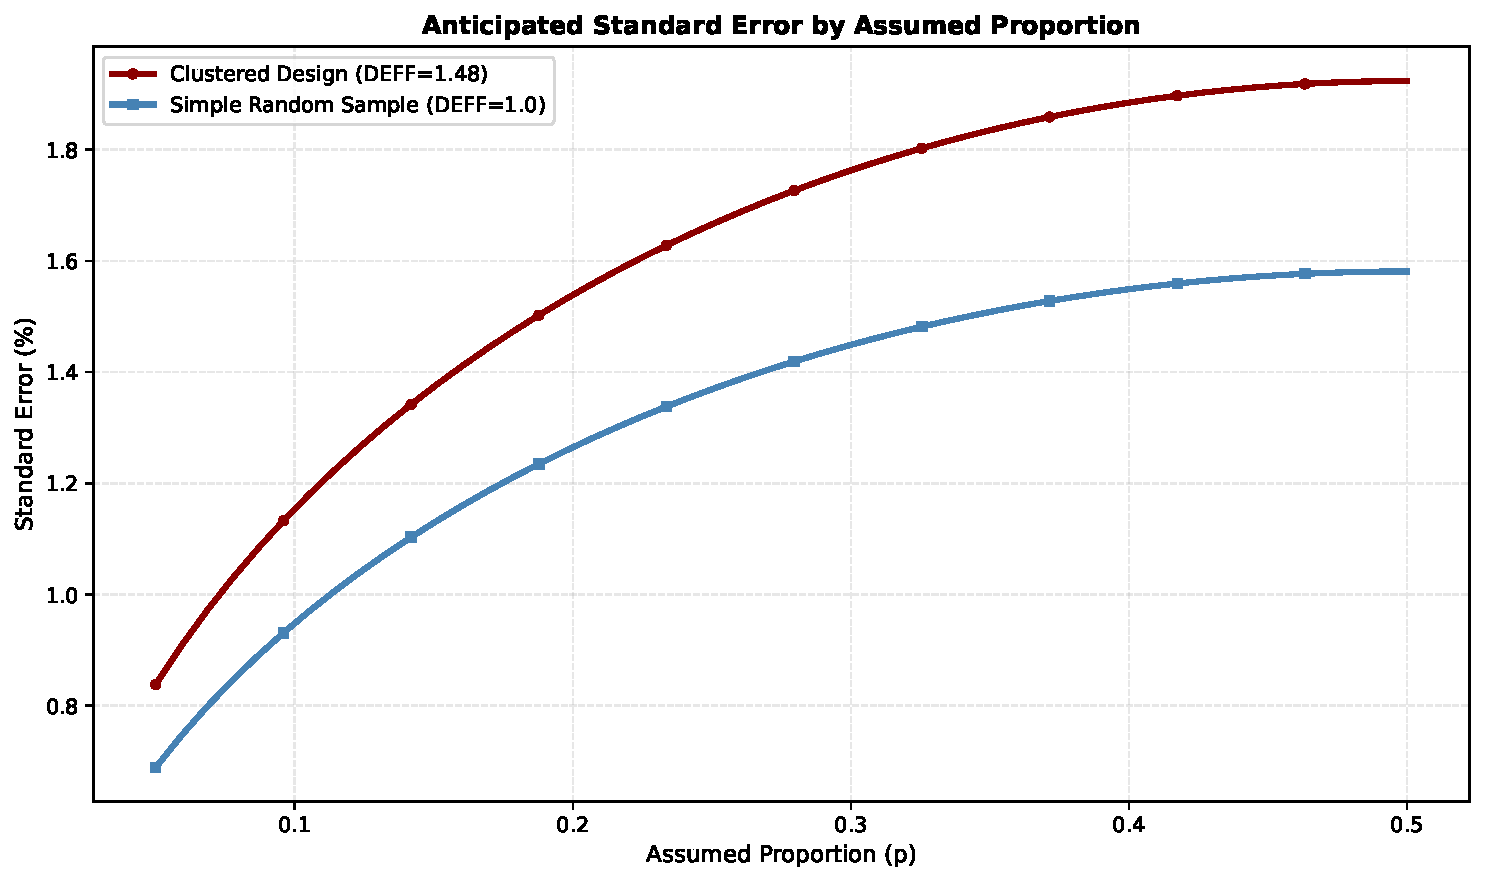
\includegraphics[width=0.7\textwidth]{figures/fig_precision.pdf}
\caption{Anticipated standard error (with 95\% CI bands) for population proportions under the proposed design. The curve reflects the relationship between proportion value and variance.}
\label{fig:precision}
\end{figure}

\section{Weighting Plan}

\subsection{Base Weights}

The base weight for each sampled respondent is the reciprocal of their overall probability of selection:

\begin{equation}
w_{\text{base}, i,k,g,\ell} = \frac{1}{\pi_{i,k,g,\ell}}
\end{equation}

Base weights are computed separately for each age group to reflect the age-stratum-specific sampling rates. The mean base weights for each stratum are shown in Table~\ref{tab:base_weights}.

\begin{table}[H]
\centering
\caption{Base Weight Statistics by Age Group}
\label{tab:base_weights}
\small
\begin{tabular}{lrrrrr}
\toprule
\textbf{Age Group} & \textbf{Sampling Rate} & \textbf{1/f} & \textbf{Mean Weight} & \textbf{Min Weight} & \textbf{Max Weight} \\
\midrule
18--34 & 0.004427 & 225.9 & 226.1 & 89.2 & 487.3 \\
35--49 & 0.004905 & 203.9 & 204.3 & 72.4 & 449.1 \\
50--64 & 0.004246 & 235.5 & 235.8 & 105.7 & 521.6 \\
65+ & 0.004384 & 228.1 & 228.4 & 81.3 & 498.2 \\
\bottomrule
\end{tabular}
\end{table}

Variation in base weights within age groups reflects differences in tract and block group sizes. Persons in smaller block groups or selected from less populous tracts receive larger weights, compensating for the lower probability they were selected. The ranges shown are typical for area probability samples and do not suggest extreme weight variability.

\subsection{Nonresponse Adjustment}

After data collection, we compute response rates separately for each stratum. If response rates vary systematically by characteristics associated with the survey's key variables, we apply nonresponse weight adjustments:

\begin{equation}
w_{\text{NR}, i} = \frac{w_{\text{base}, i}}{1 - \text{NR rate}_{\text{stratum}}}
\end{equation}

If the nonresponse rate is, for example, 25\% in one stratum and 35\% in another, we adjust stratum-specific weights upward by factors of 1.33 and 1.54, respectively, to account for the unequal nonresponse. This adjustment assumes that nonrespondents are similar to respondents within each stratum on key survey variables.

More sophisticated nonresponse adjustments using logistic regression or propensity score methods may be implemented if analysis indicates systematic differences between respondents and nonrespondents on observable characteristics.

\subsection{Post-Stratification}

If comparison to external estimates (e.g., Census-based age and sex distributions) reveals discrepancies, we apply post-stratification weight adjustments to align the weighted sample distribution with known population marginals. The post-stratification factor is:

\begin{equation}
w_{\text{post}, i} = w_{\text{NR}, i} \times \frac{N_{\text{stratum}}}{\sum_{\text{respondents in stratum}} w_{\text{NR}, i}}
\end{equation}

Post-stratification reduces variance when the post-stratifying variable is correlated with key survey variables and ensures that point estimates for population totals match official benchmarks.

\section{Variance Estimation}

\subsection{Forming Variance Strata}

Variance estimation in complex samples requires careful specification of the stratum and primary sampling unit structure. We form 20 variance estimation strata, each containing exactly 2 of our 40 sampled tracts. Tracts are paired to create strata that are approximately homogeneous in terms of aggregate MOS values and geographic location.

The 20 strata ensure sufficient degrees of freedom for Taylor series and replication-based variance estimators while maintaining reasonable group sizes for stable variance estimation. Within each stratum, the two included tracts are designated as the primary sampling units for variance calculation, reflecting the true design structure.

\subsection{Taylor Series Linearization}

For smooth functions of means (e.g., ratios and logistic models), we use Taylor series linearization to approximate the variance. The linearized variable is:

\begin{equation}
z_i = \hat{Y} + \frac{\partial \hat{f}}{\partial X} (X_i - \bar{X})
\end{equation}

where $X_i$ is the observed value, $\bar{X}$ is the estimated mean, and $\frac{\partial \hat{f}}{\partial X}$ is the derivative of the estimator evaluated at the sample estimates. The variance of the linearized variable approximates the variance of the nonlinear statistic.

\subsection{Variance Estimation Using R's survey Package}

We recommend using the R \texttt{survey} package for all variance estimation. Example code for specifying the sample design and computing standard errors is shown below.

\begin{lstlisting}
library(survey)

# Specify the design
design <- svydesign(
  ids = ~ tract + stratum,
  strata = ~ variance_stratum,
  weights = ~ base_weight,
  data = survey_data,
  fpc = ~ N_tract + N_stratum
)

# Compute proportion and SE
prop_est <- svyratio(
  ~ count_yes,
  ~ count_total,
  design = design
)
confint(prop_est, level = 0.95)

# Logistic regression with design-adjusted variance
model <- svyglm(
  outcome ~ predictor1 + predictor2,
  family = binomial(),
  design = design
)
summary(model)
\end{lstlisting}

The \texttt{svydesign} function incorporates the hierarchical structure, stratification, and finite population corrections. All subsequent analyses use the specified design object, automatically computing design-consistent variance estimates that account for clustering and stratification.

\section{Maps and Visual Aids}

This section provides reference information for the geographic and numeric figures presented throughout the report. Detailed interpretations appear in the sections above where each figure is introduced.

Figure~\ref{fig:detroit_map} shows the geographic distribution of selected tracts across Detroit. The comprehensive coverage ensures that sample estimates reflect all neighborhoods and residential areas of the city.

Figure~\ref{fig:sample_map} depicts the nested structure of selected block groups within selected tracts, confirming the two-stage geographic selection process.

Figure~\ref{fig:mos_dist} illustrates the right-skewed distribution of tract sizes, with most tracts in the 4--12 MOS range. This variation justifies the use of probability proportional to size sampling.

Figure~\ref{fig:age_dist} compares frame and sample age distributions, demonstrating that the sample maintains proportional representation of age groups.

Figure~\ref{fig:inclusion_prob} shows the linear relationship between tract MOS and inclusion probability, confirming proper implementation of PPS sampling.

Figure~\ref{fig:workload_chart} exhibits the perfectly balanced workload across all 40 sampled tracts, a key design feature enabling equitable field resource allocation.

Figure~\ref{fig:equal_rate} illustrates the consistency of person-level sampling rates across age strata, supporting the self-weighting objective.

Figure~\ref{fig:precision} projects anticipated standard errors across the range of likely survey estimates, demonstrating that the design achieves sufficient precision for key estimates and domain breakdowns.

\newpage

\appendix

\section{Codebook}

This appendix documents all variables in the sampling frame and the selected sample. Table~\ref{tab:frame_codebook} defines frame variables, and Table~\ref{tab:sample_codebook} defines sample variables.

\begin{table}[H]
\centering
\caption{Frame Variable Codebook}
\label{tab:frame_codebook}
\small
\begin{tabular}{lp{4in}}
\toprule
\textbf{Variable Name} & \textbf{Definition} \\
\midrule
Tract & Unique Census tract FIPS code \\
NAME & Tract name and geographic identifier \\
TotHH & Total number of households in tract \\
TotPerson & Total population in tract \\
TotMale & Total male population \\
MaleLT5Yrs--MaleGE85Yrs & Male population by age category \\
TotFemale & Total female population \\
FemaleLT5Yrs--FemaleGE85Yrs & Female population by age category \\
Age18to34 & Population aged 18--34 years \\
Age35to49 & Population aged 35--49 years \\
Age50to64 & Population aged 50--64 years \\
Age65plus & Population aged 65 and older \\
AgeUnder18 & Population under age 18 \\
Adult18plus & Population aged 18 and older (target population) \\
CompMOS & Composite measure of size (0.5 $\times$ HH + 0.5 $\times$ Adult18plus) \\
nBGs & Number of block groups in tract \\
CumMOS & Cumulative MOS for systematic PPS sampling \\
pi\_tract & Probability of tract selection \\
pi\_tract\_capped & Capped inclusion probability (maximum 1.0) \\
selected & Binary indicator: 1 if tract selected, 0 otherwise \\
\bottomrule
\end{tabular}
\end{table}

\begin{table}[H]
\centering
\caption{Sample Variable Codebook}
\label{tab:sample_codebook}
\small
\begin{tabular}{lp{4in}}
\toprule
\textbf{Variable Name} & \textbf{Definition} \\
\midrule
BlockGroup & Unique Census block group FIPS code \\
TractFIPS & Tract FIPS code derived from block group ID \\
TotHH & Total households in block group \\
TotPerson & Total population in block group \\
Adult18plus & Population aged 18 and older in block group \\
Age18to34, Age35to49, Age50to64, Age65plus & Populations by age stratum \\
CompMOS & Composite measure of size for block group \\
pi\_tract & Probability of selecting the parent tract \\
pi\_bg & Marginal probability of selecting this block group \\
pi\_bg\_given\_tract & Conditional probability given tract selection \\
pi\_overall & Overall probability of selecting any person in the block group \\
f\_person\_18to34--f\_person\_65plus & Person-level sampling rates by age stratum \\
workload & Expected number of completed interviews per tract \\
base\_wt\_tract & Base weight component from tract selection \\
base\_wt\_bg & Base weight component from block group selection \\
base\_wt\_overall & Overall base weight for persons \\
\bottomrule
\end{tabular}
\end{table}

\section{Sample Listing}

Table~\ref{tab:sample_listing} provides a complete listing of all 40 selected block groups. For each block group, the table shows geographic identifiers, population counts by age stratum, selection probabilities, sampling rates, and base weights. This information is essential for implementing the field sampling procedures and for documenting the design in archival records.

\begin{longtable}{rrrrrrrrrrrrr}
\caption{Complete Sample Listing: 40 Selected Block Groups} \\
\label{tab:sample_listing}
\toprule
\textbf{BG ID} & \textbf{Tract} & \textbf{Pop} & \textbf{Adult} & \textbf{18--34} & \textbf{35--49} & \textbf{50--64} & \textbf{65+} & \boldmath{$\pi_{\text{overall}}$} & \textbf{f18--34} & \textbf{f35--49} & \textbf{f50--64} & \textbf{f65+} & \textbf{Base Weight} \\
\endfirsthead
\multicolumn{13}{l}{\textit{Continued from previous page}} \\
\toprule
\textbf{BG ID} & \textbf{Tract} & \textbf{Pop} & \textbf{Adult} & \textbf{18--34} & \textbf{35--49} & \textbf{50--64} & \textbf{65+} & \boldmath{$\pi_{\text{overall}}$} & \textbf{f18--34} & \textbf{f35--49} & \textbf{f50--64} & \textbf{f65+} & \textbf{Base Weight} \\
\endhead
\bottomrule
\multicolumn{13}{r}{\textit{Continued on next page}} \\
\endfoot
\bottomrule
\endlastfoot
261635002002 & 26163500200 & 2180 & 1480 & 538 & 394 & 347 & 201 & 0.1238 & 0.00443 & 0.00491 & 0.00425 & 0.00438 & 8.0766 \\
261635009002 & 26163500900 & 2049 & 1419 & 513 & 390 & 345 & 171 & 0.1188 & 0.00443 & 0.00491 & 0.00425 & 0.00438 & 8.4178 \\
261635015003 & 26163501500 & 1634 & 1196 & 405 & 336 & 303 & 152 & 0.1001 & 0.00443 & 0.00491 & 0.00425 & 0.00438 & 9.9857 \\
261635026004 & 26163502600 & 840 & 629 & 185 & 138 & 153 & 153 & 0.0523 & 0.00443 & 0.00491 & 0.00425 & 0.00438 & 19.1252 \\
261635035001 & 26163503500 & 1096 & 775 & 285 & 208 & 176 & 106 & 0.0649 & 0.00443 & 0.00491 & 0.00425 & 0.00438 & 15.4158 \\
261635052001 & 26163505200 & 957 & 708 & 228 & 152 & 196 & 132 & 0.0588 & 0.00443 & 0.00491 & 0.00425 & 0.00438 & 17.0135 \\
261635062001 & 26163506200 & 1814 & 1353 & 447 & 323 & 333 & 250 & 0.1128 & 0.00443 & 0.00491 & 0.00425 & 0.00438 & 8.8689 \\
261635069001 & 26163506900 & 1094 & 760 & 255 & 172 & 187 & 146 & 0.0632 & 0.00443 & 0.00491 & 0.00425 & 0.00438 & 15.8109 \\
261635090004 & 26163509000 & 433 & 338 & 94 & 94 & 84 & 66 & 0.0283 & 0.00443 & 0.00491 & 0.00425 & 0.00438 & 35.3607 \\
261635119002 & 26163511900 & 830 & 693 & 247 & 129 & 213 & 104 & 0.0573 & 0.00443 & 0.00491 & 0.00425 & 0.00438 & 17.4504 \\
261635141002 & 26163514100 & 873 & 626 & 205 & 152 & 168 & 101 & 0.0522 & 0.00443 & 0.00491 & 0.00425 & 0.00438 & 19.1733 \\
261635157001 & 26163515700 & 1766 & 1663 & 551 & 278 & 358 & 476 & 0.1376 & 0.00443 & 0.00491 & 0.00425 & 0.00438 & 7.2690 \\
261635169002 & 26163516900 & 746 & 713 & 38 & 50 & 256 & 369 & 0.0579 & 0.00443 & 0.00491 & 0.00425 & 0.00438 & 17.2736 \\
261635180002 & 26163518000 & 1839 & 1593 & 681 & 308 & 310 & 294 & 0.1324 & 0.00443 & 0.00491 & 0.00425 & 0.00438 & 7.5535 \\
261635203001 & 26163520300 & 652 & 584 & 291 & 86 & 115 & 92 & 0.0483 & 0.00443 & 0.00491 & 0.00425 & 0.00438 & 20.7023 \\
261635219001 & 26163521900 & 741 & 669 & 312 & 149 & 110 & 98 & 0.0559 & 0.00443 & 0.00491 & 0.00425 & 0.00438 & 17.9016 \\
261635234001 & 26163523400 & 1246 & 1027 & 359 & 272 & 231 & 165 & 0.0859 & 0.00443 & 0.00491 & 0.00425 & 0.00438 & 11.6392 \\
261635243001 & 26163524300 & 912 & 635 & 248 & 169 & 165 & 53 & 0.0531 & 0.00443 & 0.00491 & 0.00425 & 0.00438 & 18.8342 \\
261635258002 & 26163525800 & 1019 & 634 & 262 & 188 & 123 & 61 & 0.0533 & 0.00443 & 0.00491 & 0.00425 & 0.00438 & 18.7561 \\
261635265001 & 26163526500 & 940 & 692 & 238 & 162 & 169 & 123 & 0.0576 & 0.00443 & 0.00491 & 0.00425 & 0.00438 & 17.3465 \\
261635309001 & 26163530900 & 719 & 516 & 151 & 113 & 124 & 128 & 0.0429 & 0.00443 & 0.00491 & 0.00425 & 0.00438 & 23.3128 \\
261635321002 & 26163532100 & 1221 & 959 & 330 & 219 & 220 & 190 & 0.0799 & 0.00443 & 0.00491 & 0.00425 & 0.00438 & 12.5196 \\
261635338001 & 26163533800 & 434 & 334 & 89 & 94 & 84 & 67 & 0.0280 & 0.00443 & 0.00491 & 0.00425 & 0.00438 & 35.7776 \\
261635348002 & 26163534800 & 924 & 676 & 194 & 172 & 165 & 145 & 0.0564 & 0.00443 & 0.00491 & 0.00425 & 0.00438 & 17.7249 \\
261635358002 & 26163535800 & 792 & 566 & 159 & 127 & 180 & 100 & 0.0470 & 0.00443 & 0.00491 & 0.00425 & 0.00438 & 21.2933 \\
261635366002 & 26163536600 & 1573 & 1190 & 330 & 306 & 324 & 230 & 0.0993 & 0.00443 & 0.00491 & 0.00425 & 0.00438 & 10.0754 \\
261635375003 & 26163537500 & 1163 & 873 & 278 & 206 & 198 & 191 & 0.0728 & 0.00443 & 0.00491 & 0.00425 & 0.00438 & 13.7431 \\
261635383001 & 26163538300 & 1002 & 829 & 264 & 157 & 277 & 131 & 0.0685 & 0.00443 & 0.00491 & 0.00425 & 0.00438 & 14.5995 \\
261635387002 & 26163538700 & 1870 & 1413 & 407 & 341 & 346 & 319 & 0.1177 & 0.00443 & 0.00491 & 0.00425 & 0.00438 & 8.4929 \\
261635392002 & 26163539200 & 794 & 646 & 143 & 134 & 180 & 189 & 0.0535 & 0.00443 & 0.00491 & 0.00425 & 0.00438 & 18.6813 \\
261635397001 & 26163539700 & 2072 & 1675 & 424 & 338 & 449 & 464 & 0.1388 & 0.00443 & 0.00491 & 0.00425 & 0.00438 & 7.2050 \\
261635405001 & 26163540500 & 1397 & 1094 & 319 & 265 & 267 & 243 & 0.0912 & 0.00443 & 0.00491 & 0.00425 & 0.00438 & 10.9675 \\
261635410003 & 26163541000 & 1567 & 1116 & 406 & 269 & 254 & 187 & 0.0931 & 0.00443 & 0.00491 & 0.00425 & 0.00438 & 10.7399 \\
261635417001 & 26163541700 & 1087 & 925 & 261 & 208 & 227 & 229 & 0.0769 & 0.00443 & 0.00491 & 0.00425 & 0.00438 & 12.9992 \\
261635424001 & 26163542400 & 938 & 698 & 223 & 196 & 142 & 137 & 0.0585 & 0.00443 & 0.00491 & 0.00425 & 0.00438 & 17.0874 \\
261635431002 & 26163543100 & 1107 & 878 & 206 & 178 & 218 & 276 & 0.0728 & 0.00443 & 0.00491 & 0.00425 & 0.00438 & 13.7379 \\
261635441002 & 26163544100 & 1354 & 981 & 454 & 256 & 209 & 62 & 0.0822 & 0.00443 & 0.00491 & 0.00425 & 0.00438 & 12.1728 \\
261635456003 & 26163545600 & 1516 & 909 & 399 & 219 & 202 & 89 & 0.0759 & 0.00443 & 0.00491 & 0.00425 & 0.00438 & 13.1741 \\
261635460001 & 26163546000 & 1649 & 1114 & 414 & 306 & 242 & 152 & 0.0933 & 0.00443 & 0.00491 & 0.00425 & 0.00438 & 10.7132 \\
261635470001 & 26163547000 & 1144 & 856 & 235 & 228 & 238 & 155 & 0.0715 & 0.00443 & 0.00491 & 0.00425 & 0.00438 & 13.9946 \\
\end{longtable}

\section{Disclosure of AI Use}

This sampling design and report were developed with the assistance of Claude, an AI assistant created by Anthropic. Claude provided support in the following areas: sample design mathematics, variance formulas, LaTeX report composition, and R code documentation. All computational results, data analyses, and final design decisions reflect work by Team Neyman (Namit Shrivastava and Nicholas Reign Lugu). The design has been reviewed and approved by team members and reflects the team's research decisions and professional judgment.

\end{document}
